%%==================================================
%% chapter04.tex for NWPU Bachelor Thesis
%% Encoding: UTF-8
%%==================================================

\chapter{实现}
\label{chap:Implementation}
之前的章节阐述了文件系统接口的逻辑设计,本章将继续描述文件接口的具体实现方法。
对于上层的FAT文件系统模块,主要负责在逻辑上完成需求的各项功能,是文件接口的核心。
该模块与具体硬件层无关,故具有良好的可移植性和拓展性。然而要实现一个文件系统接口并进行实验验证,硬件层必不可少,
而SD卡的驱动模块就负责联系文件系统模块与硬件层,控制数据的物理传输。

\section{预定义}
\label{sec:Defination}
鉴于「int」类型在不同CPU\footnote{32位CPU和64位CPU的「int」长度不一,并且,不同编译器也可能出现对「int」的不同定义。}上有不同的定义长度,
为了尽可能满足可移植性的要求,本工程仅使用以下三种固定长度的数据类型,
同时,为了使用方便,本工程将不同长度的数据类型分别重新定义为「BYTE」、「WORD」和「DWORD」:
\begin{lstlisting}[language={C}, caption={数据类型重定义}]
//长8位
typedef unsigned char	BYTE;
//长16位
typedef unsigned short	WORD;
//长32位
typedef unsigned long	DWORD;
\end{lstlisting}

接下来可以定义所需的结构体了。由于本工程不是很复杂,所以文件系统(FatFS)的结构体中除了包含FAT32文件系统参数信息之外,
还包含了文件的信息(比如文件指针、文件大小、起始簇号等)。
\begin{lstlisting}[language={C}, caption={文件系统数据类型}]
typedef struct {
	BYTE	fs_type;        //FAT文件系统的类型(FAT12、FAT16或FAT32)
	BYTE	csize;          //簇大小(单位为扇区)
	DWORD	n_fatent;       //FAT表的总记录数(卷可用簇数加2)
    DWORD   fatsize;        //单张FAT表的大小
	DWORD	fatbase;        //首张FAT表的起始地址(单位为扇区)
	DWORD	dirbase;        //根目录区起始地址(单位为扇区)
	DWORD	database;       //数据区起始地址(单位为扇区)
    //FSINFO项
    WORD    fsi_sec;        //FSINFO 的扇区号
    DWORD   freecont;       //空闲簇数
    DWORD   nxtfree;        //下个空闲簇号
    // 文件项
    BYTE    flag;           //文件的标志位(判断打开关闭)
    DWORD	fptr;           //文件的读写指针
	DWORD	fsize;          //文件大小
	DWORD	org_clust;      //文件起始簇号
	DWORD	curr_clust;     //文件当前簇号
	DWORD	curr_sect;		//文件当前扇区号
} FATFS;
\end{lstlisting}
除此外,还定义了目录项(Directory Entry)的结构体。
\begin{lstlisting}[language={C}, caption={目录项数据类型}]
typedef struct {
	WORD	index;          //该目录项在目录表的序号
	BYTE	fn[12];         //文件名
	DWORD	sclust;         //目录表的起始簇号
	DWORD	clust;          //目录表的当前簇号
	DWORD	sect;           //目录表的当前扇区号
} DIR;
\end{lstlisting}

\section{文件系统相关函数的实现}
\label{sec:Function}
对于FAT文件系统模块,需要始终维护一个FATFS类型的全局变量的指针$fs$,$fs$指向的变量将记录并及时更新文件系统的信息。
\subsection{挂载文件系统}
\label{sec:Mount}
在文件接口要求的所有功能中,挂载文件系统总是第一步\footnote{SD的插拔检测过于容易,本章暂且按下不表,下章会再次说明。}要做的,
其他的后续操作只有在文件系统成功挂载的情况下才变得可行。
而挂载文件系统的第一步,是能够正确无误\footnote{此处的正确无误指在逻辑上无错误,至于物理上的传输无误由底层的驱动模块保证。}的读入「DBR」扇区,
因为多数磁盘的「MBR」扇区才是物理上的$0^{th}$扇区,在「MBR」与「DBR」之间存在一定数目的隐藏扇区。因此,首要任务是分辨「MBR」和「DBR」,
同时正确定位「DBR」的位置。本模块不需对扇区进行逐块比较,而是采用一种更加快捷的办法:
\begin{balgo}{定位「DBR」扇区}{algo:dbr}
\begin{algorithmic}
\Require buff[512]\Comment{内存开辟一块缓冲池,单位字节,用来暂存从磁盘读出的数据}
\If{WORD(buff $+$510) $\neq$  0xAA55 }\Comment{是否是启动扇区}
    \State \Return Error: Not Boot Sector
\ElsIf{buff[0] $\neq$ (0xEB $and$ 0xE9)} \Comment{「DBR」的首字节必须是0xEB或0xE9}
    \State \Return DWORD(buff $+$454)\Comment{从0x1C6(454)开始的4个字节是「DBR」扇区号}
\EndIf
\end{algorithmic}
\end{balgo}

其中,「WORD(addr)」和「DWORD(addr)」分别指采用大端模式从$addr$读出16位数(字)和32位数(双字)。
通过算法\ref{algo:dbr}就可以取得正确的「DBR」扇区号了,之后要做的就是读入启动扇区(Boot Sector),
并更新$*fs$的各项信息。而且,由于使用的文件系统是FAT32,还要在读入逻辑上的$1^{st}$扇区,这个扇区记录了FSINFO的相关信息,
同样需要在$*fs$中进行更新,具体判断和定位「DBR」扇区的方法以及挂载文件系统的流程可见图\ref{fig:fsmount}。
\begin{figure}[!htb]
    \centering
    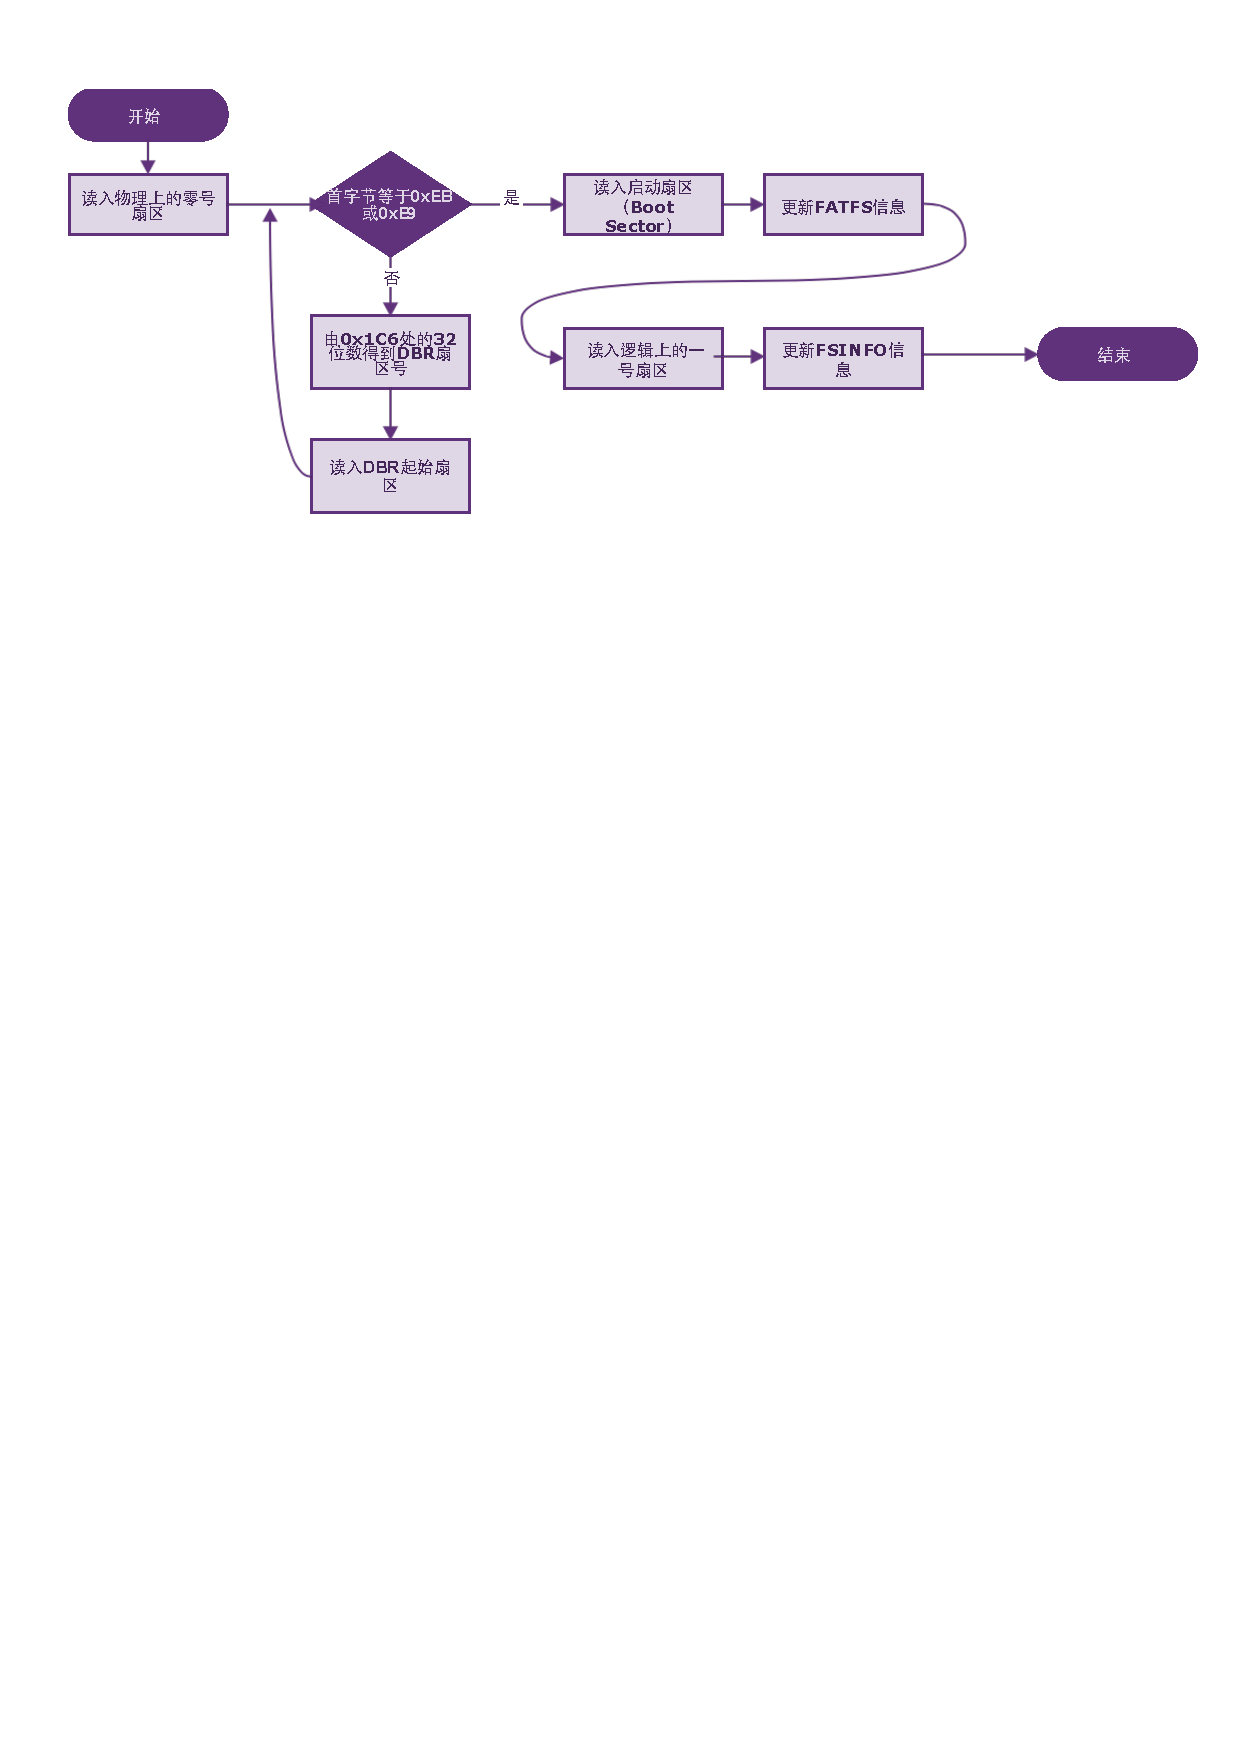
\includegraphics[width=1.0\textwidth]{chap3/mount.pdf}
    \\
    \caption{挂载文件系统}\label{fig:fsmount}
\end{figure}

\subsection{文件的创建与删除}
\label{sec:Create}
创建删除文件是相对而言比较复杂的操作,因为它们不仅设计的对FAT表的操作,还涉及到了对目录表的操作。
文件的创建或删除,要先在父目录中查找文件,对于创建操作,若查找返回无文件则可以新建文件,包含了在父目录表中登记目录项记录和在FAT表中新建簇链两个操作;
对于文件的删除操作,若查找成功则可以删除文件,包含了在父目录表中删除目录项记录和在FAT表中删除簇链。
具体的判断流程见图\ref{fig:crtdel}。
\begin{figure}[!htb]
    \centering
    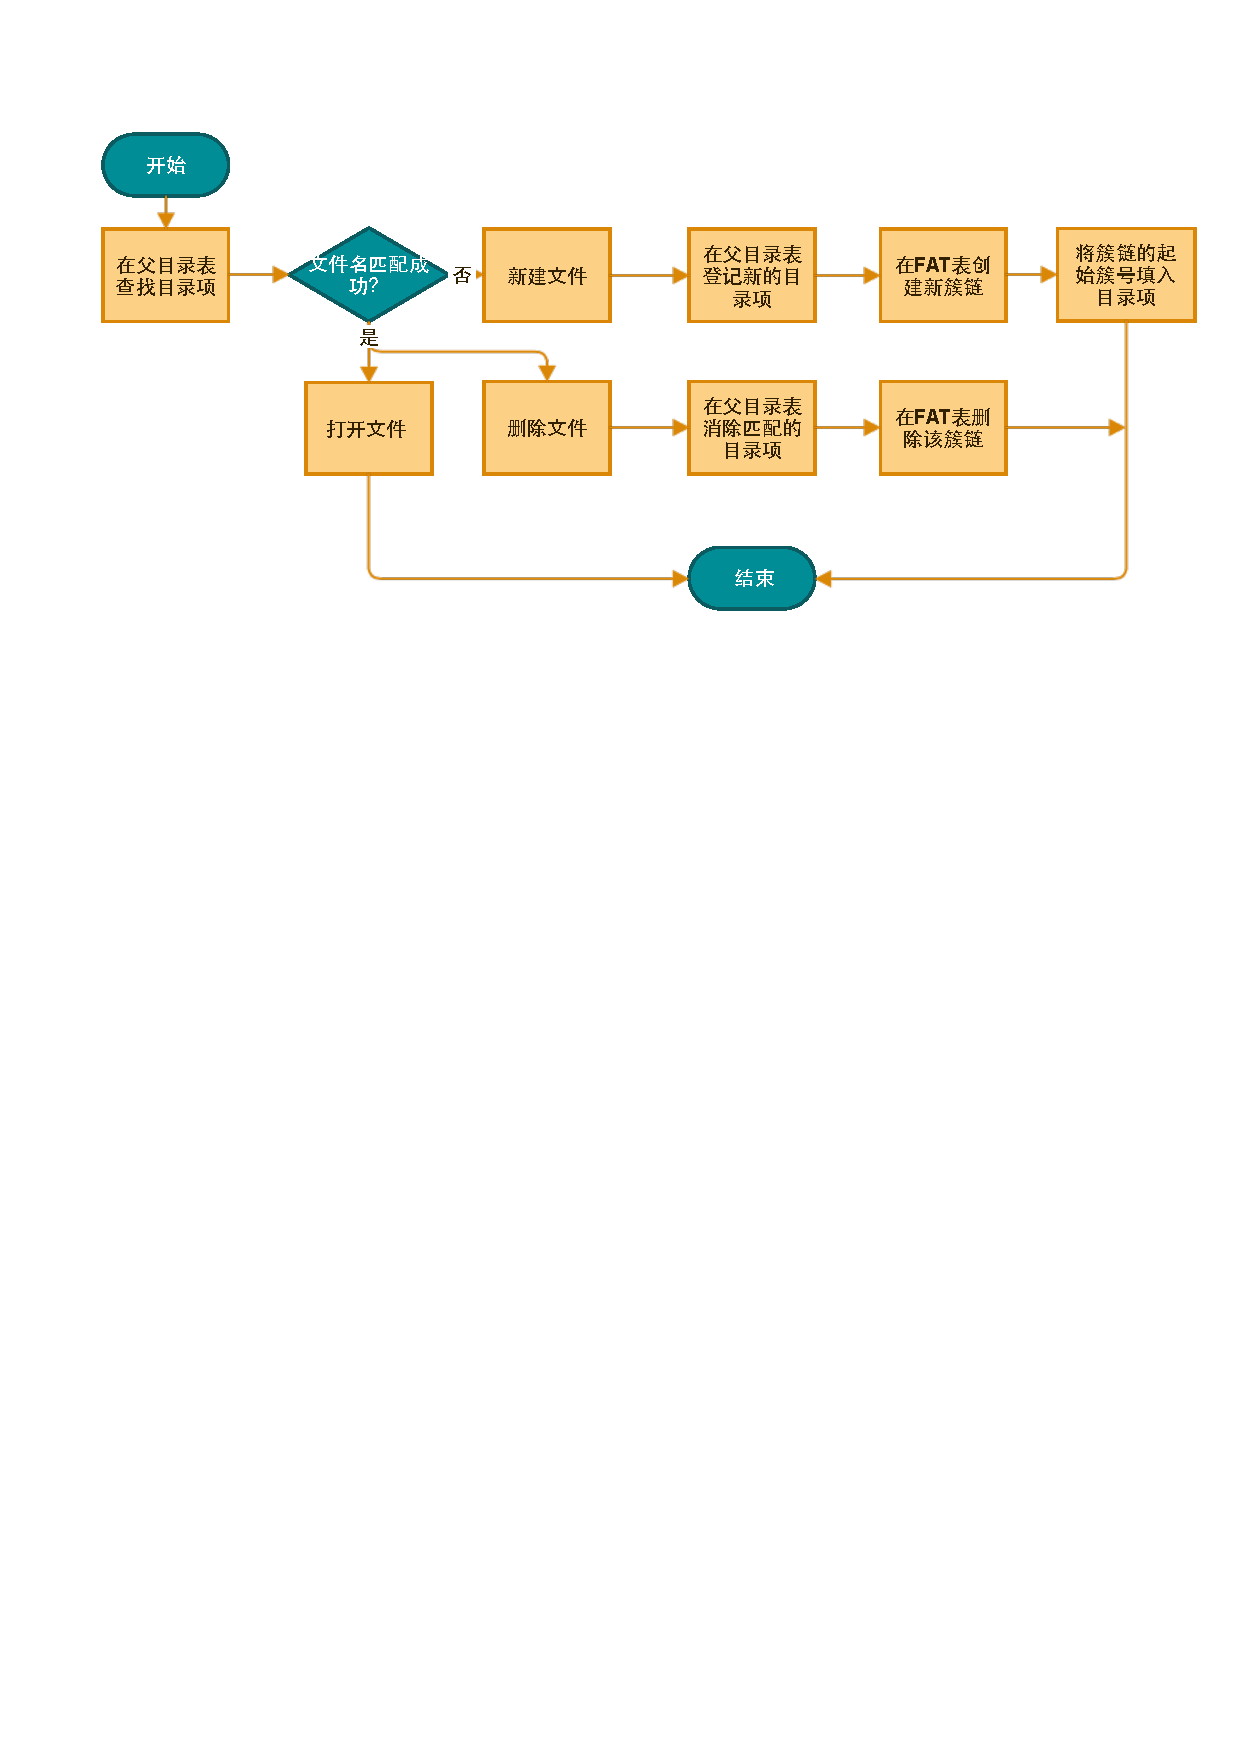
\includegraphics[width=1.0\textwidth]{chap3/creatdel.pdf}
    \\
    \caption{创建或删除文件}\label{fig:crtdel}
\end{figure}
\subsubsection{目录操作}
\label{sec:dir}
首先,实现对目录表的操作,即在一张目录表(本工程中,始终是在根目录操作)中登记(Register)一条32字节大小的目录项或者删除一条记录。
无论是登记还是删除,都需要先在该目录表上进行查找,查找是采用文件名匹配的方式,当找一个空闲的可用目录项时,结束查找。

在查找目录项的过程中,要用到两个操作「Rewind」和「Next」。顾名思义,「Rewind」就是将目录表上的指针复位,使其回到目录表的起始目录项处,
「Next」就是将指针前进32字节,即将指针指向下一个目录项。由于FAT32文件系统的规定,扇区字节数必须能够被「512」整除,且每簇扇区数都是2的整数次幂,
因此目录项总能够与扇区或者簇的边界对齐,任一条目录项都不会横跨两个扇区。
\begin{balgo}{指针越界判断}{algo:boundry}
\begin{algorithmic}
\Require Index \Comment{目录项在目录表中的序号,从$0$开始}
\If{Index $\bmod{(\frac{512}{32})} = 0$}\Comment{到达扇区边界?}
    \If{Index $\div ( \frac{512}{32} )=$ fs->csize} \Comment{到达簇边界?}
    \State Need to change the cluster
    \Else\Comment{不需换簇}
    \State Need to switch to next sector
    \EndIf
\Else\Comment{尚在同一扇区}
    \State No exceeding
\EndIf
\end{algorithmic}
\end{balgo}
因此通过算法\ref{algo:boundry}可以判断指针是否以及到达扇区或簇的边界,若只是到达扇区边界,只需从磁盘读入相邻的下一扇区,覆盖掉当前内存缓冲池「buff」即可。
但如果是到达簇边界,则需要进入FAT表的相应簇号记录项处,沿着簇链取得下一簇号,具体情况在第\ref{sec:fat}节描述。

在查找目录项时,采用文件名匹配方式,即将文件名当做一个字符串进行匹配。在FAT32文件系统的规范中,短文件名「SFN」的格式必须是「8+3」,即文件名长8字节,
扩展名长3字节,并且鉴于FAT文件系统对字母大小写不敏感,因此存入目录项中的文件名一律都是大写字母。
这样一来,通过<string.h>提供的「memcmp」函数就可以很容易地实现文件名匹配操作。
但是,对空闲目录项的判别并不是文件名匹配,而是判断该目录项的第一个字节是否为「0xE5」或「0x00」。
如果指针指向的目录项首字节为「0xE5」,表明该目录项空闲可用;如果是「0x00」,则表明之后的包含此目录项在内的所有目录项都空闲可用。

一旦找到一条可用的空闲目录项,对于登记目录项操作,此时需要将准备好的『文件名』写入32字节目录项前11个字节,紧跟的字节一般都会填入「0x20」,
即表明该目录项是普通文档而非目录。至于『时间戳』,可以不填写,默认置零即可。『文件大小』在新登记的目录项中是零,之后可能会根据写入的数据大小而更改。
最重要的部分是目录项的『起始簇号』,这个32位的簇号会分为高16位和低16位分别填入,至于簇号怎样得到,具体参见\ref{sec:fat}。
至于删除记录项,仅需将首字节置为「0xE5」,同时要取得相应的『起始簇号』,具体参见\ref{sec:fat}。

\subsubsection{FAT操作}
\label{sec:fat}
如前所述,对于文件创建操作,当在目录表中登记了一条新记录后,只需再进入FAT表新建一个簇链并将相应簇号录入该目录项即完成了文件的创建操作。
至于文件的删除,当在目录表中删除了一条记录同时取得其起始簇号后,还要进入FAT表删除相应的簇链。

因此,现在将问题转变成了新建簇链和删除簇链。
新建簇链要先查找一个可用的空闲簇号,
这里会用到FAT32文件系统所特有的数据结构FSINFO,通过其记录的「fs->nxtfree」,指明了当前FAT表最后一个分配的簇号。
查找空闲簇号时只需从「fs->nxtfree」处开始遍历整张FAT即可,如果该值为「0xFFFFFFFF」表明此值无效,此时要从「2」号簇开始遍历。
一旦找到一个空闲簇号,在其处写入「0x0FFFFFFF」\footnote{「EOC」标记}即表示该簇已被占用,且是当前簇链的最后一个簇号,然后将该簇号返回即可,
对于创建文件操作,这个簇号就是其目录项的『起始簇号』,也是这个文件数据存储的起始簇号。

至于删除簇链,进入FAT表并直接定位到给定的簇号处,接着开始遍历以这个簇号起始的簇链,遍历的同时删除每一个遍历到的簇号
(删除簇号就是将「0x00000000」作为值写入),直到这条簇链遍历结束。至此,簇链的删除就完成了。

在对FAT操作的过程中,只能操作低28位,高4位不可变更。即写入FAT表记录项的值时,要保留其高四位(通过『或』操作和『与』操作完成),
而读出值时要忽略高四位,一般将其清零即可。

\subsection{文件的打开与关闭}
\label{sec:Open}
文件的打开操作实际已经包含在文件的创建操作中,当文件不存在时,文件的打开操作退化为文件的创建操作;当文件已经存在时,
只需读入目录表中的该文件的相关目录项记录的信息,如文件大小、起始簇号等,之后将文件的读写指针清零,同时置文件的标志位有效,即表明文件已打开。

文件的关闭操作相类似,文件不存在时返回错误信息;文件存在时,最主要的是将文件标志位清零,然后将其他信息如读写指针、文件大小等清零即可。

\subsection{文件的读写}
\label{sec:Read}
对文件进行读写数据是本文件接口最主要的功能,并且读写操作互为逆操作,其中向文件中写数据相比读数据要更复杂一些。
读写文件函数需要的参数包括:缓存区地址、未传输字节数和总共要传输的字节数,其中,未传输字节数初始值为零。
读文件内的数据到缓存,首先要求判断文件是否以及打开,具体通过$*fs$中的文件标志位进行判断。

在文件成功打开的情况下,判断尚未传输的字节数是否大于「fs->fsize」与「fs->fptr」的差,如果是,则说明当前文件容量不足以供这么多的字节进行写入或读出,
如果当前操作是读操作,那么提供的要求读出的字节数超限,直接截断,按照文件大小读取数据;
但是,如果当前操作是写操作,当待写字节数超限时,需要更新文件大小「fs->fsize」的值,并且,每当分配的簇空间不足时,要进行续接簇链操作,
以取得更多的簇供数据写入。

具体的读写文件过程如图\ref{fig:freadflow}所示。
\begin{figure}[!htbp]
    \centering
    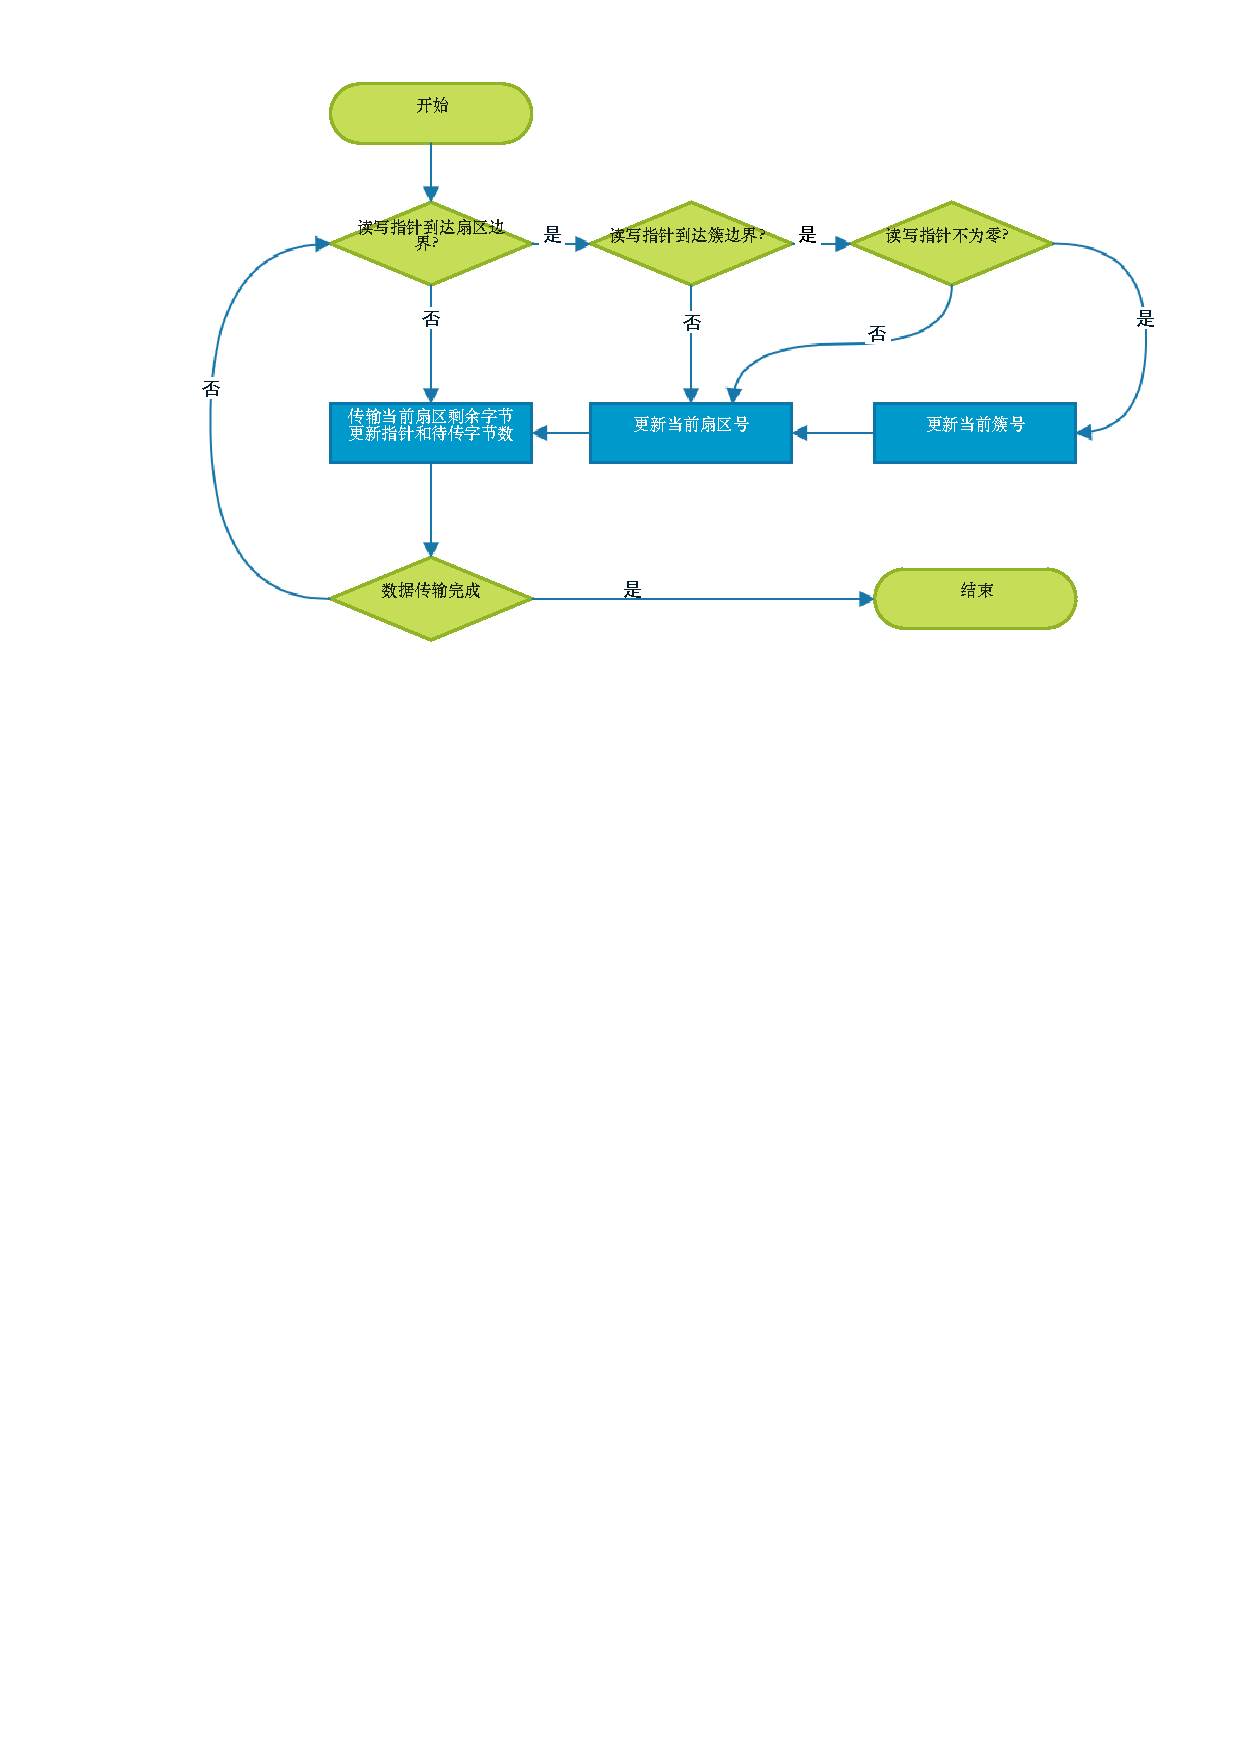
\includegraphics[width=1.0\textwidth]{chap3/freadh.pdf}
    \\
    \caption{读写文件}\label{fig:freadflow}
\end{figure}
读写文件整体上差不多,主体循环结构都如图\ref{fig:freadflow},主要差别在于其中的「更新当前簇号」操作。
在读文件操作中,更新簇号就是循着文件的簇链找到下一个簇号并使之成为当前簇号,赋值给「fs->curr\_clust」即可;
但在写文件操作中,更新簇号后还要求进一步判断:如果该簇号合法,则继续;如果该簇号为「EOC」标记,表明当前簇链已到末尾,
此时需要在该簇链的基础上创建簇链,即续接簇链,和之前的方法一样,找到一个空闲簇号,用其取代需要续接的簇链的最后一个簇号的值(「EOC」标记),
同时将该空闲簇号的值设为「EOC」标记即可,如此就完成了续链的操作。

\subsection{读写指针的重定位}
\label{sec:Ptr}
有时不想从文件的起始字节读写数据,而是想要向文件追加数据(从末尾写),或者修改文件中的某一部分数据(从文件中一个偏移值处写数据),此时,
就需要重定位文件的读写指针「fs->fptr」。
指针重定位函数不仅仅是重设了「fs->fptr」的数值,更重要的是,在重设指针的偏移字节后,要同时更新指针所在的扇区和簇号,以支持接下来的读写操作。

更新指针后,首先要通过「cnt $=$ (fs->fptr $\div$ fs->csize $\div$ 512)」求出在读写指针前有「cnt」个簇。
如果发现当前指针所在的簇为文件的第一个簇(cnt = $0$),
则将簇号回溯为文件的起始簇号即可。如果指针所在簇不是第一个簇(cnt $\neq 0$),那么需要通过起始簇号沿着簇链前进「cnt」次以取得相应簇号。

\section{底层函数的实现}
\label{sec:Diskread}
对于SD卡的驱动层模块,定义了一个32位长的全局变量$BASE$,用来记录逻辑扇区号与物理扇区号的差值。
当上层模块调用函数「disk\_offset()」时,将$BASE$的值设为「MBR」扇区「0x1C6」开始的32位数。
此后,对于上层的FAT模块,只需告诉底层模块逻辑扇区号即可,后者会在读写扇区前将之转化为物理扇区号。

\subsection{SD卡初始化并进入SPI模式}
\label{sec:Initial}
SD卡上电后处于SD模式,如果在接收复位命令(CMD0)期间片选信号(CS)保持低电平,那么将进入SPI模式。
如果卡检测到需求为SD模式则不会对复位命令做出响应,否则将切换至SPI模式同时回应SPI模式的R1。

返回SD模式的唯一方法是重新上电。在SPI模式中,所有SD卡协议的机器将不可见,而SD协议下的命令总是可用的。
图\ref{fig:specflow}显示了SPI模式的初始化序列。

初始化完成后需要通过CMD58的回应得到SD卡的CCS信息。当SD卡接受CMD8并且完成初始化后CCS有效。CCS=0表示其为标准容量卡,
CCS=1为大容量卡(SDHC或SDXC)。

\begin{figure}[!htbp]
    \centering
    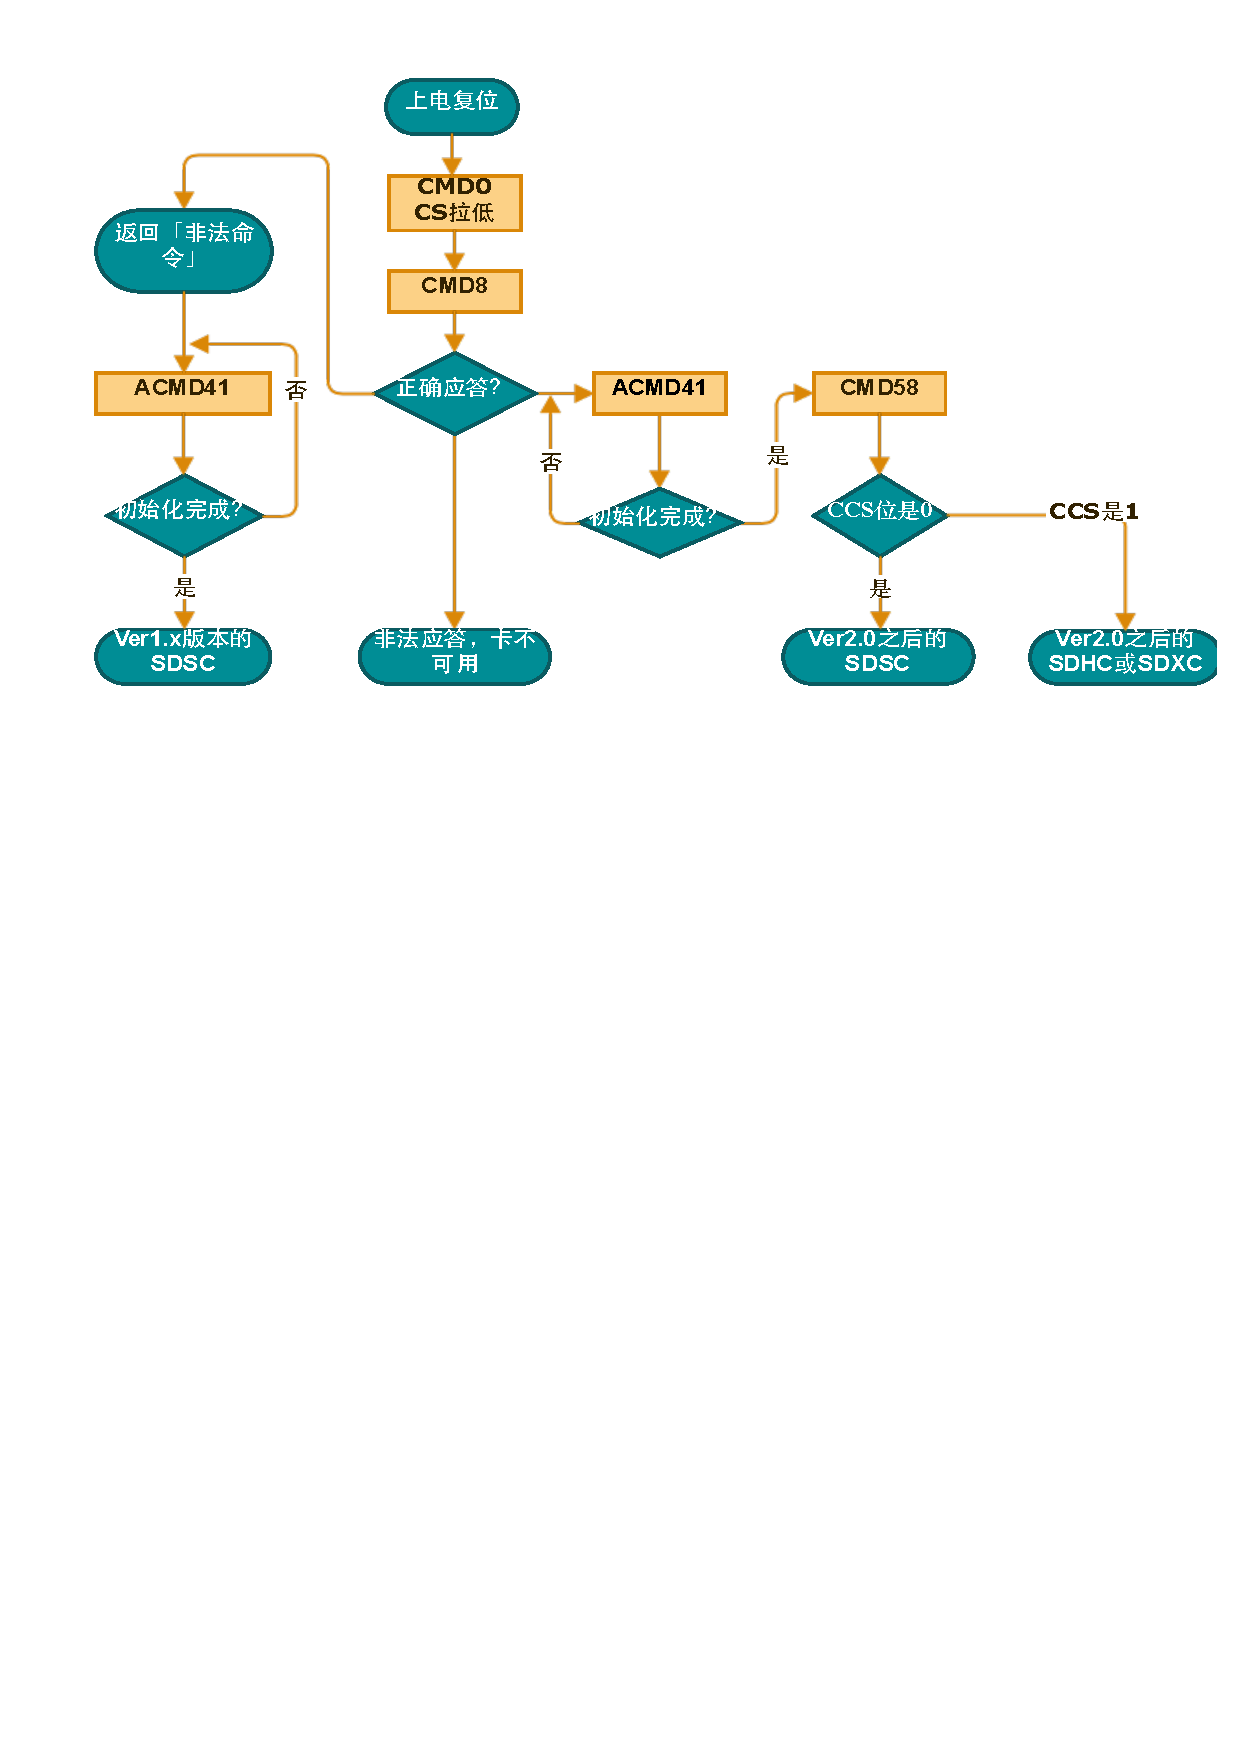
\includegraphics[width=1.0\linewidth]{chap3/specflowh.pdf}
    \\
    \caption{SPI模式初始化流程} \label{fig:specflow}
\end{figure}

初始化时需要采用低速初始化,此时SPI的时钟频率不能超过$400Khz$,本工程使用的是$200Khz$。
初始化结束后可以提升至高速。
发送命令后收到的响应如果不正确,可以循环发送命令直到收到正确应答。对于ACMD41而言,
由于其包含了两个命令(CMD55、ACMD41),故两个命令必需都收到正确应答才算响应正确,否则,两个命令都需要循环发送。

\subsection{SD卡读写扇区}
\label{sec:Sectorrw}
在SPI模式下读写扇区,首先要判断SD卡是SDSC还是SDHC/SDXC,对于前者,32位读写地址指的字节地址;对于后者,该地址指的是扇区地址。
为了同时兼容这两种卡,在该模块也定义了一个全局变量「SD\_Type」,在SD卡初始化函数中进行赋值,合法值为「SDSC」、「SDHC」和「SDXC」。
扇区读写函数通过下面方式选择字节地址或扇区地址。
\begin{lstlisting}[language={C}, caption={判断SD类型以选择合适的地址单位}]
if(*SD_Type != V2HC){
    sector = sector << 9;
}
\end{lstlisting}

由于不同文件系统的每簇扇区数各不相同,处于最大兼容性和效率性的考量,扇区读写函数都使用了单数据块传输的方式(512字节),因为一旦使用多数据块传输,
很可能出现跨簇的情况,这是非常危险的,因为本底层模块不具备跨簇的能力。
并且,本模块在写扇区之前,预先进行了擦除操作,这相比未擦除时的写入速度有了很大的提高。

\section{小结}
\label{sec:Sum3}
本章具体描述了整个文件接口各个模块的各功能函数的具体实现过程和方法,重点在与FAT文件系统模块的各个函数的实现过程,
为了增强可读性,极少使用伪代码描述,多数都采用自然语言的描述方式,与流程图相结合,具体阐述了功能的实现。

